\documentclass{beamer}

\input{../Haust2015glærur}

\title{Tölvunarfræði 1a}
\subtitle{Vika 9, seinni fyrirlestur}

\begin{document}

\begin{frame}
\titlepage
\end{frame}

\section{Inngangur}

\begin{frame}{Í síðasta þætti\ldots}
\begin{itemize}
 \item Innlestur skráa
 \item Skipanalínan (óvart, ekki til prófs)
 \item Páskaegg í Matlab (líka óvart, ekki til prófs)
\end{itemize}
Kafli: 9.1
\end{frame}

\begin{frame}[fragile]{Gömul fyrirlestraræfing}
Látum þetta forrit reikna summu:
\begin{minted}[frame=lines]{matlab}
fid = fopen('subjexp.dat');
if fid ~= -1
    while ~feof(fid)
        line = fgetl(fid);
        [number, character] = strtok(line);
        fprintf('%.2f%s\n', str2double(number), character)
    end
else
    error('Ekki tókst að opna skrá');
end
fclose(fid);
\end{minted}
\end{frame}

\begin{frame}[fragile]{Gömul fyrirlestraræfing}
Ný lykkja:
\begin{minted}[frame=lines]{matlab}
mySum = 0;
while ~feof(fid)
    line = fgetl(fid);
    [number, character] = strtok(line);
    mySum = mySum + str2double(number);
end
\end{minted}
Breytan \texttt{mySum} mun nú innihalda summuna eftir lok keyrslu.
\end{frame}

\begin{frame}[fragile]{Gömul fyrirlestraræfing}
Spurt var:
\emph{Föll á borð við \texttt{fopen} gefa ákveðið skilagildi (\texttt{-1}) sem hægt er að athuga gildið á til að sjá hvort að keyrslan hafi tekist. Hvaða brögðum má beita til að athuga hvort að föll sem ekki eru með slík sérstök skilagildi hafi lent í villu?}
\pause

\vspace{1cm}
Svar: \texttt{try/catch}
\end{frame}

\section{Almenn skráarvinnsla (9.1)}

\subsection{Innlestur heillar skrár í einu}

\begin{frame}[fragile]{\texttt{textscan}}
\begin{itemize}
 \item Fallið \texttt{textscan} les alla skrána inn í hólfavigur
\begin{minted}[frame=lines]{matlab}
>> cellArray = textscan(fid, 'snið')
\end{minted}
 \item Sniðið getur innihaldið sniðslýsingar á svipaðan hátt og \texttt{fprintf}
 \item Úttakið er hólfavigur, með eitt hólf fyrir hvern dálk í skránni
\end{itemize}
\end{frame}

\begin{frame}[fragile]{Dæmi um notkun \texttt{textscan}}
\begin{minted}[frame=lines]{matlab}
>> fid = fopen('subjexp.dat');
>> cellArray = textscan(fid, '%f %c')
cellArray = 
    [5x1 double]    [5x1 char]
>> cellArray{1}'
ans =
    5.3000    2.2000    3.3000    4.4000    1.1000
\end{minted}
Í sniðslýsingunni: \texttt{f} fyrir double, \texttt{c} fyrir char
\end{frame}

\begin{frame}[fragile]{\texttt{textscan} fyrir strengi}
Hægt er að nota \texttt{textscan} fallið á streng til að skipta honum niður í hólfavigur:
\begin{minted}[frame=lines]{matlab}
>> myString = '0.45 abc 123';
>> secondCellArray = textscan(myString, '%f %s %d')
secondCellArray = 
    [0.4500]    {1x1 cell}    [123]
\end{minted}
\end{frame}

\subsection{Að skrifa í skrár}

\begin{frame}[fragile]{\texttt{fprintf} í skrá}
\begin{itemize}
 \item Aðalskipunin til að skrifa í skrár er \texttt{fprintf}
 \begin{itemize}
  \item Þetta er sama \texttt{fprintf} fall og við könnumst við
  \item Til að skrifa í skrána þarf að láta fallið fá skráarauðkenni sem fyrsta viðfang
 \end{itemize}
 \item Notkunin verður þá á borð við \verb|fprintf(fid, 'snið', breyta1, breyta2...)|
\end{itemize}
\end{frame}

\begin{frame}[fragile]{\texttt{fprintf} í skrá}
Dæmi:
\begin{minted}[frame=lines]{matlab}
fid = fopen('tilraun.txt', 'w');
for i = 1:5
    fprintf(fid, '%d: %d\n', i, randi(50));
end
fclose(fid);
\end{minted}
Ath. að hér er skráin \emph{yfirskrifuð} í hvert skipti. Til að skrifa aftast í skrá þarf að gefa \texttt{fopen} aðrar heimildir.
\end{frame}

\begin{frame}{Skráarheimildir}
\begin{center}
\begin{tabular}{ll}
\toprule
Regla&Lýsing\\
\midrule
\texttt{'r'}&Opnar skrá til lesturs\\
\texttt{'w'}&Opnar eða býr til skrá til skriftar, yfirskrifar\\
\texttt{'a'}&Opnar eða býr til skrá til skriftar, skrifar aftast\\
\texttt{'r+'}&Opnar skrá til skriftar eða lesturs\\
\texttt{'w+'}&Opnar eða býr til skrá til skriftar eða lesturs, yfirskrifar\\
\texttt{'a+'}&Opnar eða býr til skrá til skriftar eða lesturs, skrifar aftast\\
\bottomrule
\end{tabular}
\end{center}
\end{frame}

\section{Excel-skrár (9.2)}

\begin{frame}{Excel-skrár}
\begin{itemize}
 \item Matlab getur unnið með Microsoft Excel skrár
 \begin{itemize}
  \item Viðkomandi föll: \texttt{xlswrite} og \texttt{xlsread}
 \end{itemize}
 \item Getur auðveldað flutning gagna á milli kerfa
\end{itemize}
\end{frame}

\begin{frame}[fragile]{\texttt{xlswrite}}
\begin{itemize}
 \item \texttt{xlswrite} skrifar fylki í Excel skrá
 \item Dæmi: Búum til $5 \times 3$ slembifylki og skrifum það í skrána \texttt{ranexcel.xls}
\begin{minted}[frame=lines]{matlab}
>> randomMatrix = randi(100, 5, 3); 
>> xlswrite('ranexcel.xls', randomMatrix); 
\end{minted}
\end{itemize}
\end{frame}

\begin{frame}[fragile]{\texttt{xlsread}}
\texttt{xlsread} les fylki úr Excel-skrá:

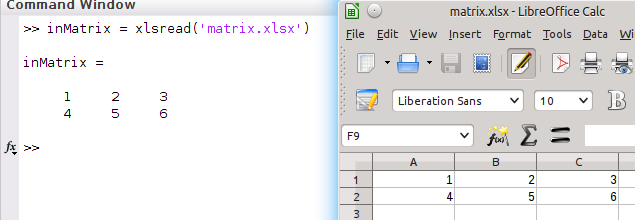
\includegraphics[width=\textwidth]{Pics/excel}

\end{frame}

\begin{frame}{Meira um Excel}
\begin{itemize}
 \item Excel-föllin hafa þó nokkra valkosti sem ekki er farið í hér
 \begin{itemize}
  \item \texttt{help xlswrite} og \texttt{help xlsread}!
 \end{itemize}
 \item Til að fá fullan stuðning þarf að vera á Microsoft Windows stýrikerfi, með Microsoft Excel uppsett
 \begin{itemize}
  \item Grundvallarvirkni er þó alltaf til staðar
 \end{itemize}
\end{itemize}
\end{frame}

\section{Að vista breytur í .mat skrár (9.3)}

\begin{frame}{Save og Load í nýjum buxum}
\begin{itemize}
 \item Hægt er að vista breytur vinnusvæðis í skrá með endinguna \texttt{.mat}
 \begin{itemize}
  \item \texttt{save} skipunin er notuð til að vista breytur í skrána
  \item \texttt{load} skipunin er notuð til að ná í þær aftur
 \end{itemize}
 \item Gagnlegt til að geyma vinnu tímabundið, t.d. til næsta vinnudags
 \item Galli: \texttt{.mat} skrár eru binary-skrár, önnur forrit en Matlab geta ekki lesið þær
\end{itemize}
\end{frame}

\begin{frame}[fragile]{Dæmi}
\begin{minted}[frame=lines]{matlab}
>> m = randi([1, 10], 2, 2) % Býr til slembifylki
m =
     2    10
     5     8
>> save vinnusvæði % Vistað í skrána vinnusvæði.mat
>> clear % breytunni m hent
>> load vinnusvæði % Breytunni m hlaðið inn aftur
>> m
m =
     2    10
     5     8
\end{minted}

\end{frame}



\begin{frame}[fragile]{Fyrirlestraræfing}
\begin{columns}
\column{0.6\textwidth}
\begin{enumerate}
 \setcounter{enumi}{3}
 \item Skrifið forrit sem les inn tölur úr skránni \texttt{subjexp.dat} og reiknar út summu þeirra talna í fyrri dálkinum þar sem stafurinn í seinni dálkinum er \texttt{'a'}.
 \item Skrifið hitastigstöfluna til hægri í skrá, þannig að hver lína í skránni innihaldi lýsingu á borð við
\begin{verbatim}
Klukkan 0 var hitinn 12.5C
\end{verbatim}
\end{enumerate}
\column{0.4\textwidth}
\begin{center}
\begin{tabular}{ll}
\toprule
Klst&$C^\circ$\\
\midrule
0&12.5\\
3&12.4\\
6&12.3\\
9&12.8\\
12&13.4\\
15&14.0\\
18&13.1\\
21&12.8\\
\bottomrule
\end{tabular}
\end{center}
\end{columns}
\end{frame}

\begin{frame}{Miðmisserispróf: Einstök dæmi}
Stigahlutfall:

Dæmi 1: 0.68\\
Dæmi 2: 0.88\\
Dæmi 3: 0.72\\
Dæmi 4: 0.76\\
Dæmi 5: 0.68\\
Dæmi 6: 0.79\\
Dæmi 7: 0.57\\
Dæmi 8: 0.68\\
\end{frame}


\end{document}
